\chapter{Marco Conceptual}\label{cap2}


En este capítulo se describen los conceptos y definiciones que le otorgan un marco de referencia teórico y formal al trabajo desarrollado. Como eje principal se estudian los grafos, específicamente sus propiedades con respecto a la representación gráfica de éstos. A continuación se explican los problemas subyacentes que se analizarán, aquellos de complejidad temporal NP, específicamente el problema de \emph{crossing number}. Finalmente, se da un panorama sobre las técnicas utilizadas para el desarrollo de los algoritmos: los \emph{algoritmos evolutivos} y su subcategoría, \emph{algoritmos genéticos}, incluyendo la especificación de cada paso para llevar a cabo su implementación.

\section{Teoría de Grafos}
\label{sec:teoria_grafos}
La teoría de grafos es un rama que estudia las propiedades de los grafos. Concibe formalismos para representarlos de manera matemática, como también de forma gráfica. En esta sección presentaremos las definiciones  formales básicas, en cuanto a los grafos como   estructura matemática,  como también de su representación visual. Asimismo se enunciarán algunos resultados sobre la estructura. Para los lectores interesados en conceptos avanzados en el tema se recomienda leer \cite{gersting2007mathematical,bondy1976graph,godsil2013algebraic,bollobas2013modern,nishizeki2004planar}.


\begin{definition}\label{defgrafo}\cite{bondy1976graph,gersting2007mathematical}
Un grafo es una tupla  ordenada de tres elementos  $G=(V,E,\psi)$, donde $V$  es un conjunto no  vacío de vértices o nodos, $E$ es un conjunto de aristas o arcos  y $\psi$ es  una función que asocia cada arista en $E$ con un par no ordenado de vértices en $V$.
\end{definition}
En este trabajo, se considerarán  grafos finitos,  esto es,  $V$ y $E$ son conjuntos finitos, a menos que se establezca explícitamente lo  contrario. 

Bajo  la definición \ref{defgrafo}, el arco denotado con $(x,y)$ es equivalente al arco  denotado $(y,x)$,  siendo  $x,y\in V$ los  puntos extremos del arco. Diremos que $x$ e $y$ son  nodos adyacentes si existe el arco $(x,y)$. Dos arcos se consideran adyacentes  si tienen un punto extremo en común \cite{bollobas2013modern}.

A continuación se  extiende la definición \ref{defgrafo}, para considerar arcos con dirección.

\begin{definition}\label{defgrafodirigido}\cite{gersting2007mathematical} 
Sea  $G=(V,E,\psi)$ un grafo. Se dice que $G$ es  un  {\em grafo  dirigido} si la función  $\psi$ asocia a cada arista en  $E$ con un {\em par  ordenado} $(x,y)$ de vértices en $V$, donde $x$ es el punto inicial e $y$ es el punto terminal de la arista. 
\end{definition}

Las definiciones de nodos y arcos adyacentes se extienden para la definición \ref{defgrafodirigido}.

\begin{definition}\cite{gersting2007mathematical}\label{defgradovertice}
Sea  $G=(V,E,\psi)$ un grafo. Decimos que el {\em grado de un vértice $v\in V$} es el número de arcos en los que $v$ es un punto extremo.
\end{definition}

\begin{definition}\cite{gersting2007mathematical}
Sea  $G=(V,E,\psi)$ un grafo. Decimos que $G$ es {\em completo} en el que  todo par de nodos o vértices  distintos son adyacentes.
\end{definition}

Un grafo puede ser utilizado para representar información como la interconexión en una red de computadoras, un circuito VSLI o el modelado conceptual de un sistema de información (UML\cite{eichelberger2003uml,auer2007explorative} u ORM\cite{halpin2005orm}) o de una base de datos (Entidad-Relación\cite{chen1988entity}).


La representación gráfica  de un grafo es  una clase de visualización de la información representada en la estructura. 

%\subsection{Aplicaciones de grafos}
%Pueden utilizarse los grafos para diversas aplicaciones. Una de principal interés es la visualización de modelos conceptuales, permitiendo representarlos ante una notación particular de cada tipo de modelado.
%imagenes de modelos conceptuales (uml, er, orm)

\subsection{Estilos de Representación Gráfica de Grafos}
\label{sec:estilos_de_dibujado}

Los grafos pueden ser representados en forma visual como un diagrama que consiste de una colección de objetos que se corresponden con los vértices del grafo y  un conjunto de segmentos lineales que se corresponden con los arcos que conectan los objetos.

Así, un grafo puede ser dibujado  sobre un plano, donde  sus vértices se representan como pequeños círculos en el diagrama y sus aristas como líneas que conectan tales círculos. 

De este modo, para dibujar un grafo se debe posicionar cada vértice sobre un punto $(x,y)$ en  el plano, y luego, unirlos mediante líneas según correspondan sus aristas. Dependiendo del estilo que se utilice,  los aristas pueden dibujarse como líneas rectas, curvas o por cadenas poligonales (líneas articuladas) \cite{nishizeki2004planar}.
 
\subsubsection{Dibujo Planar}
Un dibujo planar de un grafo es aquel en el que no hay intersección entre ningún par de aristas. Es posible dibujar un grafo de manera planar o no planar, pero no todos los grafos tienen un dibujado planar. Un grafo que admite al menos un dibujo planar es llamado {\em grafo planar}.

\begin{figure}
	\centering
	\subfigure[Grafo dibujado de manera planar]{
		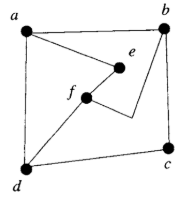
\includegraphics[width=0.33\textwidth]{imagenes/grafo_planar_1.png}
		\label{subfig:ejemplo_dibujado_planar}
	}
	\subfigure[El mismo grafo dibujado de manera no planar]{
		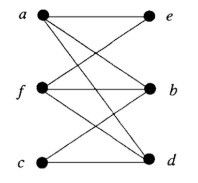
\includegraphics[width=0.33\textwidth]{imagenes/grafo_no_planar_1.png}
		\label{subfig:ejemplo_dibujado_no_planar}
	}
	\caption{Ejemplo de grafo planar. Dibujado de manera planar y no planar \cite{nishizeki2004planar}.}
	\label{fig:ejemplo_dibujado_planar}
\end{figure}
\subsubsection{Dibujo con Polilíneas}
Un gráfico con  polilíneas \cite{nishizeki2004planar} es  un dibujo de  un grafo en el que cada arco del grafo es representado por  una cadena poligonal. Una cadena poligonal es un línea continua que está compuesta de una serie de uno  o más segmentos  de líneas conectadas. En la Figura \ref{fig:ejemplo_dibujado_polilineas}\
 se  muestra un dibujo de un grafo con polilíneas. El punto en el que el arco  cambia su  dirección es  llamado  punto de doblez.

Este estilo de dibujo provee una gran flexibilidad, ya que pueden   aproximar dibujos con arcos curvos. Sin embargo, puede ser dificultoso para el ojo, seguir un arco con tres  o más puntos de doblez.

\begin{figure}
	\begin{center}
		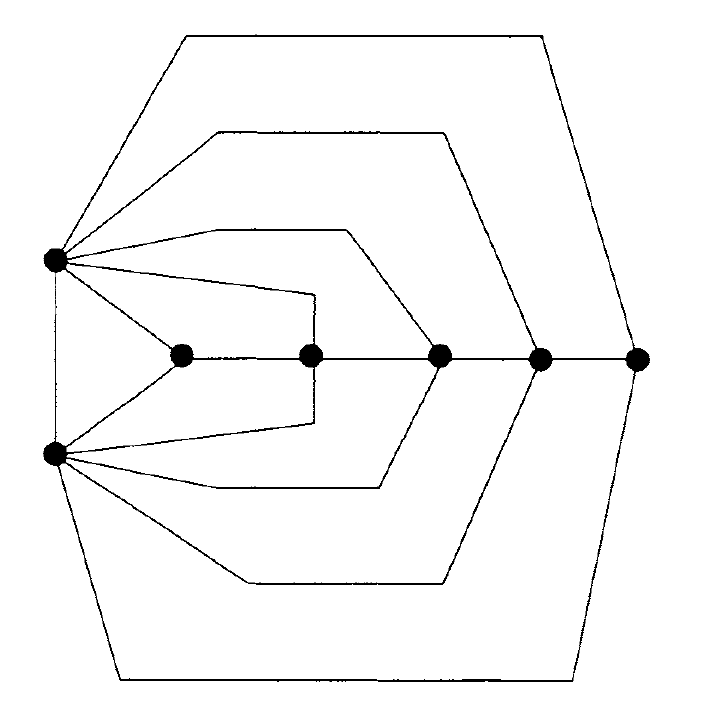
\includegraphics[scale=0.3]{imagenes/GrafoPolilinea.png}
	\end{center}
	\caption{Ejemplo de grafo dibujado con polilíneas \cite{nishizeki2004planar}.}\label{fig:ejemplo_dibujado_polilineas}
\end{figure}



\subsubsection{Dibujo como Diagrama de Arcos}
\label{sec:dibujado_diagrama_de_arcos}

Un Diagrama de Arcos \cite{Wat02} es un estilo con el  que se dibuja un grafo, en el que los vértices del grafo se ubican sobre  una línea en el plano  Euclídeo y los arcos se dibujan como  semicírculos, sobre alguno de los dos  semiplanos delimitados por la línea o bien pueden ser segmentos de la línea, siempre que conecten vértices que son consecutivos en la recta.
En la Figura \ref{fig:arcdiagram_ejemplo} se muestra un ejemplo con 7 nodos.

\begin{figure}[h]
	\centering
	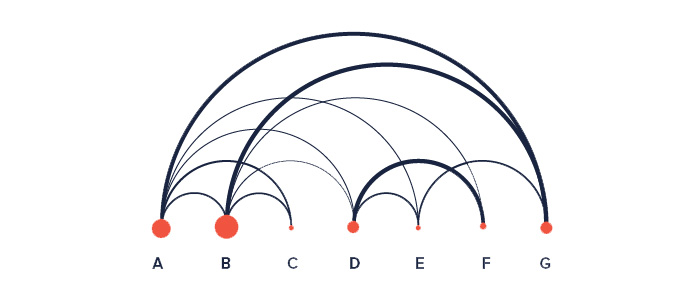
\includegraphics[width=12cm]{imagenes/diagrama-de-arco.jpg}
	\caption{Ejemplo de un diagrama de arcos.}
	\label{fig:arcdiagram_ejemplo}
\end{figure}

%imagen de grafo arc diagram

\subsection{Propiedades de la Representación Gráfica de Grafos}
\label{sec:propiedades_dibujado_grafos}
Los grafos pueden dibujarse de diversas formas, pero al momento de dibujar un grafo para un uso específico se consideran una variedad de propiedades. Éstas brindan medidas para fortalecer ciertas características, que quieran destacarse o mejorarse en  un dibujo, para así hacerla más intuitiva según su dominio. Por ejemplo, si el grafo corresponde a un circuito VLSI, luego estaremos interesados en un dibujo planar, cuyo número de puntos de doblez  sea el mínimo posible, ya que estos puntos aumentan el costo. Por otra parte, es importante evitar desperdiciar espacio valuable en el chip, por lo que  el área del dibujo deberá ser  lo más  pequeña posible.

A continuación se presentan, algunas propiedades en el dibujo de los grafos, que se introducen en  \cite{nishizeki2004planar} y que serán de interés en este trabajo.\\

\begin{property}{\bf\em  Área}\\
	Es el área que ocupa el plano donde se dibuja el grafo. Si el área es de gran tamaño, entonces tendremos que visualizarlo mediante muchas páginas o desplazarnos sobre el plano. En cambio, si disminuimos la resolución se vuelve más dificultoso de leer. En este sentido, se busca una relación de aspecto favorable entre el tamaño y la resolución.
\end{property}

\begin{property}{\bf\em Cruces de Arcos}\\
	Los cruces o intersecciones de arcos abren a posibles confusiones de lectura, por lo que en cualquier dibujo, siempre se busca disminuir lo más posibles la cantidad de cruces.
\end{property}



\section{Problemas NP}
\label{sec:problemas_np}
Los problemas NP son aquellos que se encuentran categorizados en la clase de complejidad temporal NP (\emph{Nondeterministic Polynomial  time}). 



\begin{definition}\cite{arora2009computational}\\
La clase NP abarca el conjunto de problemas de decisión que  pueden ser resueltos en un tiempo polinomial, por una Máquina de Turing No Determinística (a partir de ahora MTND). Formalmente,
$$\text{NP} = \bigcup_{k \in  \mathbb{N}}^{}{\text{NTIME}(n^k)}$$
donde $\text{NTIME}(n^k)$ es el conjunto de problemas que pueden resolverse por una MTND en tiempo $O(n^k)$.
\end{definition}


Asumiendo la conjetura de que $P\neq NP$, es importante distinguir  los  problemas en NP que no están en la clase P, ya que este grupo es el que se considera intratable\cite{garey1979computers}.

Así, aparece la teoría de  los  problemas NP-completos, que forma una clase de equivalencia entre los lenguajes, bajo la propiedad de  ser considerados los más difíciles en NP.

\begin{definition}\label{defNP-Completo}\cite{garey1979computers}
Un lenguaje $L$ asociado a un problema de decisión es NP-completo,  si 
\begin{enumerate}
    \item $L\in NP$
    \item NP-hard: Para cada lenguaje $L^{\prime}\in NP$,  $L^{\prime}$ reduce  en tiempo polinomial a L.
\end{enumerate}
\end{definition}
Nótese,  que dos  problemas de decisión $\Pi_1$ y $\Pi_2$ que son NP-completo, son  equivalentes entre sí,  dado que por el  punto (1) de la definición \ref{defNP-Completo}, ambos están en NP y por el punto (2) deben ser reducibles entre ellos. 

La importancia de estos problemas reside en que por un lado caracterizan a los problemas más difíciles de resolver. 
Por el otro, si un problema $\Pi$  que es NP-completo, pudiera ser resuelto en tiempo polinomial con una Máquina de Turing Determinística (MTD),  esto es,  $\Pi\in P$,  entonces {\em todos} los  problemas en NP, se podrían resolver en tiempo polinomial con una MTD. En consecuencia, si  un problema  NP-completo está en P, P$=$NP.

Aún conociendo que  estos problemas de decisión son NP-completos,  es interesante estudiarlos, a fin de encontrar   una forma de resolverlos  en un tiempo asequible, ya sea bajo técnicas heurísticas o bien restringiendo el problema a casos especiales.

Existen muchos problemas en diferentes dominios que están  en esta clase.  Entre estos, se considera de interés el problema  Crossing Number, tópico de esta tesis.

\subsection{Crossing Number}
\label{sec:crossing_number}
Una de las propiedades fundamentales del dibujo de grafos (Propiedad \ref{sec:propiedades_dibujado_grafos}) es el número de cruces de arcos. Esta propiedad  es central  en áreas de Ciencias de la Computación, como lo es el diseño  de chip y el dibujo de grafos automático.


El parámetro más común para medir esta propiedad,  se define formalmente, como sigue. Dado  un grafo $G=(V,E)$,  representaremos con  $cr(G)$   al  número de cruces que tiene un dibujo de $G$.

El \emph{\bf problema de decisión   crossing number} se define como \cite{garey1983crossing} ``Dado un grafo $G$ y un número entero $K$, ¿existe un dibujo de $G$ tal que $cr(G) \leq K$?"

El correspondiente \emph{\bf problema de optimización} se define como\cite{turan1977note}:  ``Dado un grafo $G$, ¿cuál es el 
menor número de cruces necesarios para dibujar a $G$?

Esto es, el menor número entero $K$ tal que $G$ puede ser dibujado en el plano, donde no haya más de $K$ intersecciones entre los arcos graficados del conjunto $E$.


Desde su introducción \cite{turan1977note}, este problema ha sido estudiado, mostrando que  es NP-completo \cite{garey1983crossing}, aún para grafos cúbicos\cite{hlinveny2006crossing}, i.e., para grafos cuyos vértices tienen exactamente  grado 3.


\section{Algoritmos de Layout de Grafos}

La posición de cada nodo y arco en un dibujo  de un grafo  es llamado el layout del grafo, esto es, la disposición de cada elemento del grafo en el plano. Este layout puede ser realizado de manera manual, lo que significa que cada nodo y arco es ubicado por el usuario, o automáticamente, es decir que un algoritmo computa las posiciones de los nodos y arcos para producir un ``mejor'' layout. Lo que constituye un ``mejor'' layout depende del tipo de grafo, la aplicación, como también de una preferencia del usuario. Típicamente, un algoritmo de layout automático para grafos intenta lograr cumplir con uno o varios objetivos estéticos (que posiblemente tengan conflictos entre ellos). Minimizar el número de cruces de arcos, maximizar la simetría, o minimizar el área que ocupa el grafo son algunos de los objetivos estéticos posibles \cite{bohringer1990using}.

Un layout automático tiene la ventaja de aliviarle al usuario la tediosa carga del layout, pero usualmente no produce un resultado tan bueno como el que se obtiene con un layout manual. Una de las principales razones por las que sucede esto, es porque la mayoría de los algoritmos de layout automáticos no están diseñados para tomar en cuenta el significado que el usuario da a esa estructura y que llevan al layout imaginado y deseado  por el usuario. Por ejemplo, el usuario, podría desear que un nodo se encuentre a la izquierda de otro o que un grupo particular de nodos sean ubicados en forma cercana para una mejor visualización. Dado que la restricción es explícita, entonces tiene más prioridad que los objetivos estéticos del algoritmo de layout.

% The position of each
% node and edge in the graph is called the layout of
% the graph. Graph layout can either be done manually, meaning that each node and edge is placed
% by the user, or automatically, meaning that an algorithm computes the position of the nodes and edges to
% produce a “nice” layout. What constitutes a “nice”
% layout depends on the type of graph, the application, as well as on the user’s taste. Typically, an
% automatic graph layout algorithm tries to meet one
% or more (possibly conflicting) aesthetic goals. Minimizing the number of edge crossings, maximizing the
% symmetries, or minimizing the total area of the graph
% are some of the many possible aesthetic goals.
% Automatic layout has the advantage of relieving the
% user of the tedious chore of layout, but usually does
% not produce quite as good results aa a manual layout.
% One of the m’a;n reasons is that most automatic layout
% algorithms are not designed to take a user’s layout 
% constraints into account. For example, the user might
% request that one node be to the left of another or that
% a particular group of nodes be placed near each other.
% Since these constraints are specified explicitly, they
% are of higher priority than the aesthetic goals of the
% layout algorithm. 

% A linear layout, or simply a layout,of an undirected graph G = (V, E) with n =|V|vertices is a bijective function ϕ : V →[n] ={1, ...,n}. A layout has also beencalled a linear ordering [Adolphson andHu 1973], a linear arrangement [Shiloach1979], a numbering [Chinn et al. 1982] ora labeling [Juvan and Mohar 1992] of thevertices of a graph. We denote by 8(G) theset of all layouts of a graph G.

% Given a layout ϕ of a graph G =(V, E) and an integer i, we define the setL(i, ϕ, G) ={u∈V : ϕ(u)≤i}and the setR(i, ϕ, G) ={u∈V : ϕ(u)>i}. The edgecut at position i of ϕ is defined asθ(i, ϕ, G) =|{uv ∈ E :u ∈ L(i, ϕ, G) ∧v ∈ R(i, ϕ, G)}|and the modified edge cut at position i ofϕ asζ (i, ϕ, G) =|{uv ∈ E : u ∈ L(i, ϕ, G)∧v ∈ R(i, ϕ, G) ∧ ϕ(u) 6= i}|.The vertex cut or separation at position iof ϕ is defined asδ(i, ϕ, G) =|{u∈L(i,ϕ,G):∃v∈R(i,ϕ,G):uv ∈ E}|.Given a layout ϕ of G and an edge uv ∈ E,the length of uv on ϕ isλ(uv, ϕ, G) =|ϕ(u)−ϕ(v)|.


Los algoritmos de layout de grafos responden a una clase particular de problemas de optimización combinatorios, cuyo objetivo es ubicar los elementos del  grafo de entrada sobre un plano,  de manera que esta disposición sea óptima. En  particular, un layout lineal es una disposición de los nodos sobre una línea imaginaria en el plano y se define formalmente como sigue.


\begin{definition}\cite{diaz2002survey}
Un {\em layout lineal} de un grafo no dirigido $G=(V,E)$ con $n=|V|$ vértices es una función biyectiva $\varphi : V \rightarrow [n] = \{1,...,n\}$. Un layout lineal puede también ser llamado un {\em ordenamiento lineal}, una numeración o un etiquetado de los vértices de un grafo. Se denota $\phi(G)$ al conjunto de todos los layout lineales de un grafo $G$.
\end{definition}

En este ordenamiento lineal,  distinguimos los  nodos que se encuentran ubicados a derecha e izquierda de un nodo arbitrario, algunas medidas de separación entre estos conjuntos y la distancia entre los nodos de acuerdo a la ubicación en la línea.

\begin{definition}\cite{diaz2002survey}
Dado un layout lineal $\varphi$ de un grafo $G=(V,E)$ y un entero $i$, se define el conjunto $L(i,\varphi,G) = \{u \in V : \varphi(u) \leq i\}$ y el conjunto $R(i,\varphi,G) = \{u \in V : \varphi(u) > i\}$. \\

El corte por arcos en la posición $i$ de $\varphi$ es una medida definida como:

$$\theta(i,\varphi,G) = |\{uv \in E : u \in L(i,\varphi,G) \wedge v \in R(i,\varphi,G)\}|$$

y el corte modificado de arcos en la posición $i$ de $\varphi$ es la medida

$$\zeta(i,\varphi,G)=|\{ uv \in E : u \in L(i,\varphi,G) \wedge v \in R(i,\varphi,G) \wedge \varphi(u) \neq i \}|$$

El corte del vértice o la separación en la posición $i$ de $\varphi$ está definida como

$$\delta(i,\varphi,G)=|\{ u \in L(i,\varphi,G) : \exists v \in R(i,\varphi,G) : uv \in E \}|$$

Dado un layout lineal $\varphi$ de $G$ y un arco $uv \in E$, la distancia de $uv$ en $\varphi$ es

$$\lambda(uv,\varphi,G) = |\varphi(u) - \varphi(v)|$$
\end{definition}


\begin{ejemplo}
Informalmente, el layout lineal es un etiquetado de los nodos de un grafo con un número entero distintivo y consecutivo \cite{diaz2002survey}, como se muestra en la Figura \ref{fig:ejemplo_grafo_linear}.

Considerando el dibujo (a)  de la Figura  \ref{fig:ejemplo_grafo_linear} e $i=3$, $L(3,\varphi,G) = \{A,B,C\}$ y  $R(3,\varphi,G) = \{D,E,F\}$. Las medidas son:
$$\theta(3,\varphi,G) = 4 $$
$$\zeta(3,\varphi,G)=3$$
$$\delta(3,\varphi,G)=3$$
Considerando el arco $(C,D)$,  $ \varphi(C)=3$ y $ \varphi(D)=4$, la distancia entre C y D es
$$\lambda(cd,\varphi,G) = |\varphi(C) - \varphi(D)|=1$$
\end{ejemplo}



\begin{figure}
	\centering
	\subfigure[Grafo etiquetado con un layout lineal.]{
		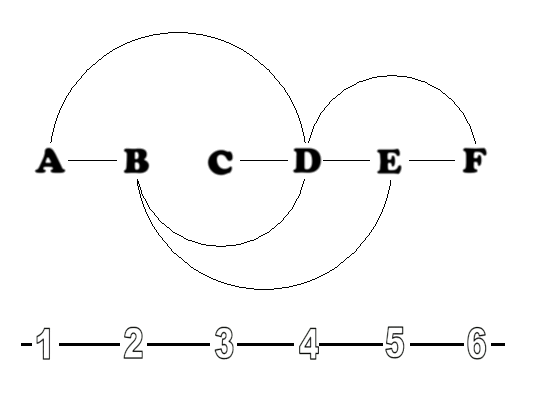
\includegraphics[width=0.39\textwidth]{imagenes/grafo_linear_2.png}
		\label{subfig:ejemplo_grafo_linear_original}
	}
	\subfigure[El mismo grafo etiquetado con otro layout lineal.]{
		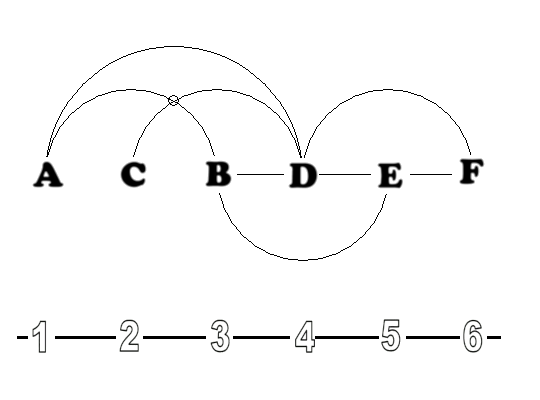
\includegraphics[width=0.39\textwidth]{imagenes/grafo_linear_1.png}
		\label{subfig:ejemplo_grafo_linear_otro_orden}
	}
	\caption{Ejemplo de layout lineal con nodos etiquetados del 1 al 6.}
	\label{fig:ejemplo_grafo_linear}
\end{figure}

Un gran número de problemas relevantes de diferentes dominios pueden ser formulados como un problema de layout de grafos. Esto incluye, optimización de redes para arquitecturas de computadoras paralelas, diseño de circuitos VLSI (Very Large-Scale Integration), gestión de información, análisis numérico, biología computacional, planificación y arqueología. Los problemas más interesantes de layout de grafos son problemas NP-Hard y sus equivalentes problemas de decisión NP-Completos, pero, para la mayoría de sus aplicaciones, es suficiente con soluciones factibles que consigan aproximadamente un costo óptimo. Como consecuencia, algoritmos aproximados y heurísticas efectivas son bienvenidas en la práctica.

% Graph layout problems are a particular
% class of combinatorial optimization problems
% whose goal is to find a linear layout
% of an input graph in such a way that a
% certain objective function is optimized. A
% linear layout is a labelling of the vertices
% of a graph with distinct integers. A large
% number of relevant problems in different
% domains can be formulated as graph layout
% problems. These include optimization
% of networks for parallel computer architectures,
% VLSI circuit design, information
% retrieval, numerical analysis, computational
% biology, graph theory, scheduling
% and archaeology. Most interesting graph
% layout problems are NP-hard and their
% decisional versions NP-complete, but, for
% most of their applications, feasible solutions
% with an almost optimal cost are sufficient.
% As a consequence, approximation
% algorithms and effective heuristics are
% welcome in practice.

\section{Algoritmos Evolutivos}
En la naturaleza, la evolución es mayormente determinada por la selección natural de diferentes individuos compitiendo en un ambiente. Aquellos individuos que son mejores son más aptos para sobrevivir, y propagar su material genético. 

La reproducción sexual permite el intercambio y re-ordenamiento de algunos cromosomas, produciendo una descendencia que contiene una combinación de la información genética de cada padre. Esta es la operación de \emph{recombinación}, que normalmente es llamada \emph{crossover} (o cruzamiento) debido a la manera en que los cromosomas se cruzan durante el intercambio. La diversidad en la población es lograda mediante la operación de \emph{mutación} \cite{grosan2011intelligent}.

Por otra parte, la codificación para la información genética (genoma) está dada en una forma que admita también la {\em reproducción asexual}, lo que resulta en una descendencia que es genéticamente idéntica a sus padres.

% In nature, evolution is mostly determined by natural selection of different individuals
% competing for resources in the environment. Those individuals that are better
% are more likely to survive and propagate their genetic material. The encoding
% for genetic information (genome) is done in a way that admits asexual reproduction,
% which results in offspring that are genetically identical to the parent.
% Sexual reproduction allows some exchange and re-ordering of chromosomes, producing
% offspring that contain a combination of information from each parent. This
% is the recombination operation, which is often referred to as crossover because of
% the way strands of chromosomes cross over during the exchange. The diversity in
% the population is achieved by mutation operation.

Estos conceptos se agrupan usualmente sobre el término \emph{Computación Evolutiva} o \emph{Algoritmos Evolutivos} \cite{back1997handbook,back1996evolutionary}, y sobre éstos encontramos particularmente el dominio de los \emph{Algoritmos Genéticos} \cite{holland1992adaptation,goldberg1989genetic}, la \emph{Programación Evolutiva}\cite{fogel1966artificial}, la \emph{Programación Genética} \cite{koza1992genetic,michalewicz1996genetic} y las \emph{Estrategias de Evolución} \cite{vent1975rechenberg,schwefel1977evolutionsstrategien}. Todos ellos comparten la misma base conceptual de simular la evolución de estructuras de individuos mediante un proceso de selección, recombinación y mutación, y de esta manera producir mejores soluciones. Los procesos dependen del desempeño percibido de las estructuras de individuos definidas por el problema particular. Este es un proceso iterativo como el que se puede ver en la Figura \ref{fig:esquema_evolutivo}.

\begin{figure}
	\centering
	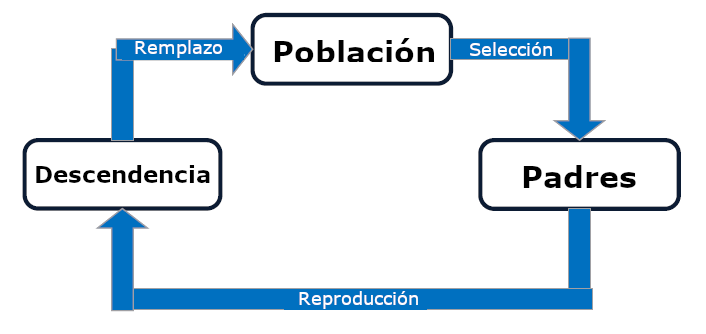
\includegraphics[width=8cm]{imagenes/esquema_evolutivo.png}
	\caption{Esquema de algoritmo evolutivo \cite{grosan2011intelligent}.}
	\label{fig:esquema_evolutivo}
\end{figure}

% Usually grouped under the term evolutionary computation or evolutionary algorithms
% [1][4], we find the domains of genetic algorithms [9], evolution strategies
% [26][27], evolutionary programming [28] and genetic programming [29].
% They all share a common conceptual base of simulating the evolution of individual
% structures via processes of selection, recombination and mutation reproduction and
% thereby producing better solutions. The processes depend on the perceived performance
% of the individual structures as defined by the problem. The procedure is
% then iterated as illustrated in Figure 14.1.

En este trabajo nos enfocaremos particularmente en  los  Algoritmos Genéticos que se describen a  continuación. 
\subsection{Algoritmos Genéticos}
\label{sec:algoritmos_geneticos}
Los algoritmos genéticos son algoritmos de búsqueda, que  están basados en la selección natural,  utilizando las similitudes del comportamiento de la genética en la naturaleza. Éstos combinan la supervivencia del más apto entre estructuras basadas en strings (cadenas de caracteres) con un intercambio de información estructurada, pero de modo aleatorio para, de esta manera, formar un algoritmo de búsqueda con un estilo similar al humano. En cada generación, un nuevo grupo de criaturas artificiales (strings) es creado y representado mediante bits procedentes de sus antecesores y nuevas partes. A pesar de ser aleatorios, los algoritmos genéticos no son simples búsquedas azarosas. Estos aprovechan la información histórica para encontrar nuevos puntos de búsqueda, de los que se espera una mejora con respecto a los anteriores \cite{goldberg1989genetic}.

Los algoritmos genéticos son probablemente el tipo de algoritmos evolutivos más utilizado y simple de implementar para cualquier tipo de problema de optimización.
El ciclo básico incluye la generación de la población inicial, evaluación de esos individuos para determinar si hemos hallado la solución al problema de optimización, la reproducción y mutación de la población  inicial y la selección de estos últimos  individuos para generar una nueva población. 

Éstos pasos presentan diferentes técnicas que involucran formas de  diseñar la representación de los individuos, los mecanismos de selección y las operaciones de variación (recombinación y mutación) \cite{grosan2011intelligent} y que se describen a continuación.

\subsubsection{Representación de Individuos}
La representación de los individuos que componen la población es uno de los pasos más importantes en el diseño de un algoritmo genético. La representación debe ser adecuada para el problema que se quiere resolver y debe consumir la menor cantidad de recursos posibles. Para un problema pueden haber múltiples posibles representaciones. Por esta razón, tenemos que determinar cuál es la más adecuada para satisfacer las necesidades y requerimientos del problema \cite{grosan2011intelligent}.

Existen tipos estándar de representación de individuos, y entre las más importantes están: %los cuales permiten utilizar la misma forma para diferentes problemas pero cambiando la interpretación que se les da. Algunas de las mas importantes son las siguientes:
\begin{itemize}
    \item Representación Binaria: cadena de bits.
    \item Representación Entera: cadena de enteros.
    \item Representación Real o Flotante: cadena de números reales o flotantes.
    \item Representación basada en Orden o Permutación: cadena de enteros que identifican el orden de los elementos.
\end{itemize}

\subsubsection{Inicialización de la Población}
El próximo paso en el desarrollo de un algoritmo genético es la inicialización de la población. Esto significa dar una semilla para generar aleatoriamente un número dado de individuos teniendo en cuenta la codificación/representación elegida. Mientras se realiza la generación, existen posibilidades de que algunos individuos puedan tener múltiples copias de sí mismos \cite{grosan2011intelligent}.

Para cada representación particular, existen diferentes técnicas para inicializar la población. Por ejemplo:

\begin{itemize}
    \item Para una representación binaria: un individuo está representado por un string con valores en $\{0, 1\}$, por lo tanto los genes deberán inicializarse con valores $0$ o $1$ de manera equiprobable.
    \item Para una representación basada en orden: el individuo esta dado por una permutación de tamaño $n$. Cada gen $i$ deberá ser inicializado con valores entre $\{1, ..., n\}$ donde el valor no debe ocurrir en las posiciones previamente inicializadas.
\end{itemize}

\subsubsection{Mecanismos de Selección}
El proceso de selección en un algoritmo genético ocurre cuando los potenciales candidatos que para ser usados en la reproducción o  crossover son seleccionados. De manera estándar, los individuos más aptos, son aquellos con mayor probabilidad de ser seleccionados \cite{grosan2011intelligent}. Para medir la aptitud de un individuo se utiliza una función  \emph{fitness},  que depende del problema y que indicará,  que tan bueno es ese  individuo dentro de la población.

Algunos de los mecanismo de selección más utilizados son:
\begin{itemize}
    \item Selección por torneo: $k$ individuos son seleccionados aleatoriamente de la población y los mejores de todos ellos son separados en otro grupo. El proceso se repite hasta que el número de padres requeridos es seleccionado de toda la población.
%     k individuals are randomly selected from the population and the best individual
% among all of them is kept in a separate set. The process is then again repeated
% until the required number of parents is selected from the whole population.
    \item Selección proporcional al fitness: la probabilidad de selección depende del fitness absoluto del individuo comparado con el acumulado del fitness absoluto del resto de la población.
%     the selection probability depends on the absolute fitness
% value of the individual compared to the absolute fitness values of the rest of the
% population.
    \item Selección por ruleta: los individuos son mapeados en segmentos contiguos de una línea imaginaria, donde cada segmento es equivalente en tamaño al fitness del individuo. Luego, un número aleatorio es generado y según el segmente donde se ubique tal número es el individuo que es seleccionado. El proceso se repite hasta obtener el número de individuos deseado.
%     the individuals are mapped to contiguous segments of a
% line, such that each individual's segment is equal in size to its fitness. A random
% number is generated and the individual whose segment spans the random number
% is selected. The process is repeated until the desired number of individuals is obtained.
    \item Selección basada en ranking: la población es ordenada a partir del valor de fitness. Tal valor no corresponde al fitness propio del individuo sino que se calcula para cada uno a partir de una función de fitness la cuál se ajusta según diferentes métodos: como ranking lineal o ranking no lineal.
%     the population is sorted according to the fitness
% (quality) values. The fitness assigned to each individual depends only on its position
% in the individual’s rank and not on the actual fitness value.
\end{itemize}

\subsubsection{Operaciones de Variación}
Las operaciones de variación principales son recombinación o \emph{crossover} y mutación. Cada una de ellas tienen formas específicas según las diferentes representaciones de individuos \cite{grosan2011intelligent}.

\begin{enumerate}
        \item{\bf Crossover o Recombinación}
El rol de la operación de \emph{crossover} es el de producir nuevos individuos combinando la información contenida en dos o más padres. Esto se logra combinando los genes de los padres. Dependiendo de la  representación de  tales genes, diferentes métodos serán utilizados \cite{grosan2011intelligent}: 

\begin{itemize}
    \item Recombinación binaria: crossover de un solo punto, crossover multipunto y crossover uniforme.
    \item Recombinación para enteros: pueden aplicarre las mismas que en la recombinación binaria.
    \item Recombinación para reales: recombinación aritmética.
    \item Recombinación para representación basada en orden:  crossover mapeado parcialmente, crossover cíclico y crossover de borde.
\end{itemize}

\item{\bf Mutación}
La mutación produce variaciones aleatorias sobre los individuos. Estas variaciones son por lo general pequeñas. La mutación se aplica a un individuo y puede producir solo un descendiente. Estas se aplican a los genes de un individuo, generalmente, con una baja probabilidad o ratio. Normalmente, los descendientes son mutados después de ser creados mediante crossover.

Como en el caso del crossover, la operación mutación toma varias formas dependiendo en la representación utilizada para los individuos y sobre cada una se pueden aplicar diferentes técnicas \cite{grosan2011intelligent}:

\begin{itemize}
    \item Mutación binaria: en esta representación solo se utilizan genes que pueden tomar dos valores, por lo que las mutaciones consisten en invertir algún gen elegido aleatoriamente con una cierta probabilidad.
    \item Mutación para enteros: reseteado aleatorio o mutación lenta.
    \item Mutación para reales: mutación uniforme o mutación no uniforme con distribución fija.
    \item Mutación para representación basada en orden: mutación basada en intercambio, mutación basada en inserción, mutación \emph{Scramble} (mezclando) o mutación basada en inversión.
\end{itemize}
\end{enumerate}
    

\subsubsection{Modelos Poblacionales}
Existen dos modelos poblacionales definidos para algoritmos genéticos:

\begin{enumerate}
    \item {\bf Modelo Generacional}
En el modelo generacional, en cada generación el algoritmo empieza con una población de tamaño $N$. Un conjunto de apareamiento de tamaño $N$ es seleccionada a partir de éste, donde algunos individuos serán seleccionados varias veces y otros no serán seleccionados en absoluto. Luego, se crean $N$ descendientes aplicando las operaciones de variación sobre éstos. Después de cada generación, la población es reemplazada por su descendencia, la cuál se transformará en la población de la siguiente generación \cite{grosan2011intelligent}.

\item {\bf Modelo de Estado Estable}
En el modelo de estado estable, la población no es reemplazada en un paso. En este caso solo $M$ ($M<N$) individuos de la población anterior son reemplazados por nuevos individuos de la descendencia. El porcentaje de la población que es reemplazado es llamada ``brecha'' generacional (o \emph{generational gap}) y es equivalente a $M/N$ \cite{grosan2011intelligent}. El algoritmo de estado estable es usualmente aplicado con $M=1$ y su correspondiente brecha generacional $1/N$ \cite{eiben2003introduction}.
% There are two main population models used by genetic algorithms:
% 1) Generational model and
% 2) Steady state model.
% Generational Model
% The generational model works as follows: in each generation the algorithm starts
% with a population of size N. A mating pool of size N is selected from this (some
% individuals will have multiple copies while other will not be selected at all). N
% offspring are further created by applying the variation operators. After each generation
% the whole population is replaced by the offspring population which will be
% the population of the next generation.
% Steady-state model
% In the steady-state model the population is not changed at once. In this case M
% (M<N) old individuals are replaced by M new individuals (from the offspring).
% The percentage of the population that is replaced is called generational gap and it
% is equal to M/N. The steady state algorithm has been widely applied especially
% with M=1 and the corresponding generational gap 1/N [2].
\end{enumerate}

\subsubsection{Selección de Supervivientes y Reinserción}
Una vez que la descendencia ha sido producida mediante la selección, recombinación y mutación de los individuos de la población anterior, el fitness de la descendencia puede ser determinado. 

Si la descendencia producida tiene menor tamaño que la población original, entonces para mantener el tamaño de la población original, la descendencia debe ser reinsertada en la población anterior. Similarmente, si no toda la descendencia es utilizada en cada generación o si se generan más individuos descendientes que el tamaño de la población anterior, entonces un esquema de reinserción debe ser utilizados para determinar que individuos existirán en la nueva población \cite{geatbx}.

Existen dos estrategias de reinserción principales:

% Once the offspring have been produced by selection, recombination and mutation
% of individuals from the old population, the fitness of the offspring may be determined.
% If less offspring are produced than the size of the original population then
% to maintain the size of the original population, the offspring have to be reinserted
% into the old population. Similarly, if not all offspring are to be used at each generation
% or if more offspring are generated than the size of the old population then a
% reinsertion scheme must be used to determine which individuals are to exist in the
% new population [12].
% There are two main reinsertion strategies:
\begin{enumerate}

\item{Reinserción Local:}\\
En la reinserción local, los individuos son seleccionados en vecindarios o grupos delimitados. La reinserción de cada descendiente toma lugar en exactamente el mismo vecindario al que pertenece. En este sentido, la localidad de la información es preservada. El padre de algún individuo es el primero en ser seleccionado para ser padre del vecindario de este \cite{geatbx}.

Para la selección de padres  a ser reemplazados y para la selección de descendencia para la reinserción existen varios esquemas posibles que toman algún criterio a partir del fitness de los individuos, o simplemente lo hacen de manera aleatoria. Un ejemplo sería: insertar la descendencia más apta  en el vecindario y reemplazar a los padres.
% In local selection, individuals are selected in a bounded neighborhood. The reinsertion
% of offspring takes place in exactly the same neighborhood. Thus, the locality
% of the information is preserved. The parent of an individual is the first selected
% parent in this neighborhood.
% For the selection of parents to be replaced and for selection of offspring to reinsert
% the following schemes are possible [12]:
    \item {Reinserción Global:}\\
Para la reinserción global existen diferentes esquemas \cite{geatbx}:

\begin{itemize}
    \item Reinserción pura: produce tanta descendencia como padres y reemplaza todos los padres por la descendencia.
    \item Reinserción uniforme: produce menos descendencia que padres y reemplaza los padres uniformemente al azar.
    \item Reinserción elitista: produce menos descendencia que padres y reemplaza los peores padres.
    \item Reinserción basada en el fitness: produce más descendencia que la necesaria y reinserta solamente los mejores individuos.
\end{itemize}

% • produce as many offspring as parents and replace all parents by the offspring
% (pure reinsertion);
% • produce less offspring than parents and replace parents uniformly at random
% (uniform reinsertion);
% • produce less offspring than parents and replace the worst parents (elitist
% reinsertion);
% • produce more offspring than needed for reinsertion and reinsert only the
% best offspring (fitness-based reinsertion).
% Pure reinsertion is the simplest reinsertion scheme. Every individual lives one
% generation only. This scheme is used in the simple genetic algorithm. However, it
% is very likely, that very good individuals are replaced without producing better
% offspring and thus, good information is lost.
% The elitist combined with fitness-based reinsertion prevents losing of information
% and is the recommended method. At each generation, a given number of the
% least fit parents are replaced by the same number of the most fit offspring. The fitness-
% based reinsertion scheme implements a truncation selection between offspring
% before inserting them into the population (i.e. before they can participate in the reproduction
% process). On the other hand, the best individuals can live for many generations.
% However, with every generation some new individuals are inserted. It is
% not checked whether the parents are replaced by better or worse offspring.
% Because parents may be replaced by offspring with a lower fitness, the average
% fitness of the population can decrease. However, if the inserted offspring are extremely
% bad, they will be replaced with new offspring in the next generation [12].

\end{enumerate}
\subsubsection{Algoritmo  Genético Básico}
Teniendo en cuenta las técnicas explicadas y el ciclo presentado en la Figura \ref{fig:esquema_evolutivo}, la forma básica de un algoritmo genético es la siguiente \cite{grosan2011intelligent}: 

\begin{enumerate}[{Paso} 1]
    \item  Generar una población aleatoria de $N$ individuos. 
     \item Evaluar cada individuo en la población utilizando la función de fitness. 
     \item Crear una nueva población repitiendo los siguientes pasos hasta que la nueva población esté completa:
% The basic form of a general genetic algorithm is:
% Step 1 Generate random population of N chromosomes.
% Step 2 Evaluate each chromosome in the population using the fitness function
% Step 3 Create a new population by repeating following steps until the new
% population is complete
\begin{enumerate}[{Paso 3.}1]
\item  Selección: selecciona dos individuos padres de la población de acuerdo con su fitness (cuanto mejor fitness, mayor es la posibilidad de ser seleccionado). 
\item  Crossover: dada un probabilidad de crossover, se cruzan a los padres para formar una nueva descendencia (hijos). Si no se realiza crossover, la descendencia es una copia exacta de los padres. 
\item  Mutación: dada una probabilidad de mutación, se mutan los individuos de la nueva descendencia en cada posición del cromosoma. 
\item  Reemplazo: se inserta la nueva descendencia en la población. \\
\end{enumerate}
% Step 3.1 Selection
% Select two parent chromosomes from a population according to their
% fitness (the better fitness, the higher the chance to be selected)
% Step 3.2 Crossover
% With a crossover probability cross over the parents to form new offspring
% (children). If no crossover was performed, offspring is the exact
% copy of parents.
% Step 3.3 Mutation
% With a mutation probability mutate new offspring at each locus (position
% in chromosome).
% Step 3.4 replacement
% Place new offspring in the new population
\item  Utiliza la nueva población generada para nuevas generaciones (iteraciones) del algoritmo. 
\item  Si la condición de finalización es satisfecha, se detiene y retorna la mejor solución de la población actual. 
\item  Si no, retorna al \emph{Paso 2}. 
% Step 4 Use new generated population for a further generation (iteration) of the
% algorithm
% Step 5 If the termination condition is satisfied, stop, and return the best solution
% in current population
% Step 6 Go to Step 2

\end{enumerate}

Este algoritmo  se utiliza en la implementación de uno de los algoritmos propuestos en esta tesis para resolver el  problema del crossing number sobre grafos dibujados como Diagramas de Arcos.
 
